% Title: gl2ps_renderer figure
% Creator: GL2PS 1.4.0, (C) 1999-2017 C. Geuzaine
% For: Octave
% CreationDate: Sun Feb  3 01:11:54 2019
\setlength{\unitlength}{1pt}
\begin{picture}(0,0)
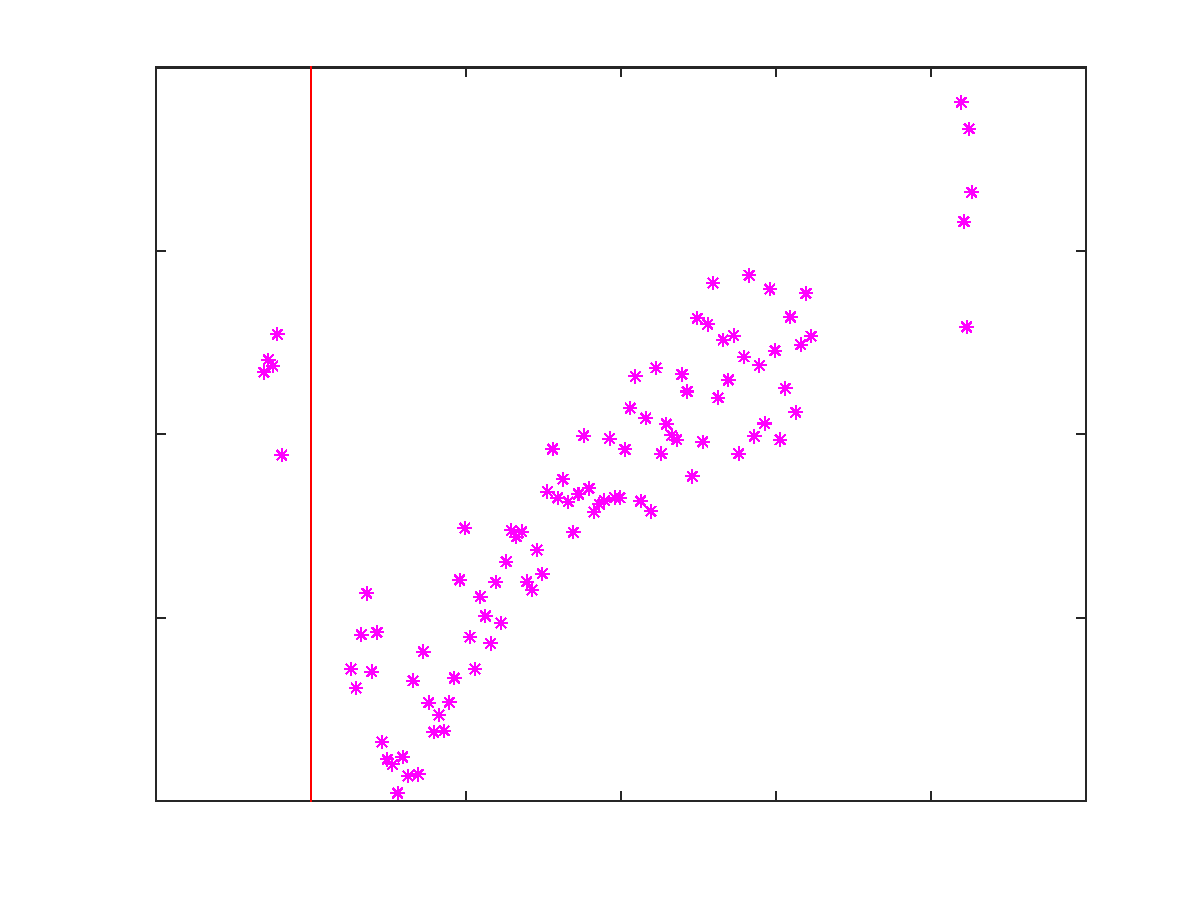
\includegraphics{/Users/Keldins/strand/plots/SAW_speeds-inc}
\end{picture}%
\begin{picture}(576,432)(0,0)
\fontsize{10}{0}
\selectfont\put(74.88,42.5039){\makebox(0,0)[t]{\textcolor[rgb]{0.15,0.15,0.15}{{-1}}}}
\fontsize{10}{0}
\selectfont\put(149.28,42.5039){\makebox(0,0)[t]{\textcolor[rgb]{0.15,0.15,0.15}{{0}}}}
\fontsize{10}{0}
\selectfont\put(223.68,42.5039){\makebox(0,0)[t]{\textcolor[rgb]{0.15,0.15,0.15}{{1}}}}
\fontsize{10}{0}
\selectfont\put(298.08,42.5039){\makebox(0,0)[t]{\textcolor[rgb]{0.15,0.15,0.15}{{2}}}}
\fontsize{10}{0}
\selectfont\put(372.48,42.5039){\makebox(0,0)[t]{\textcolor[rgb]{0.15,0.15,0.15}{{3}}}}
\fontsize{10}{0}
\selectfont\put(446.88,42.5039){\makebox(0,0)[t]{\textcolor[rgb]{0.15,0.15,0.15}{{4}}}}
\fontsize{10}{0}
\selectfont\put(521.28,42.5039){\makebox(0,0)[t]{\textcolor[rgb]{0.15,0.15,0.15}{{5}}}}
\fontsize{10}{0}
\selectfont\put(69.8755,47.5137){\makebox(0,0)[r]{\textcolor[rgb]{0.15,0.15,0.15}{{2387}}}}
\fontsize{10}{0}
\selectfont\put(69.8755,135.527){\makebox(0,0)[r]{\textcolor[rgb]{0.15,0.15,0.15}{{2388}}}}
\fontsize{10}{0}
\selectfont\put(69.8755,223.554){\makebox(0,0)[r]{\textcolor[rgb]{0.15,0.15,0.15}{{2389}}}}
\fontsize{10}{0}
\selectfont\put(69.8755,311.568){\makebox(0,0)[r]{\textcolor[rgb]{0.15,0.15,0.15}{{2390}}}}
\fontsize{10}{0}
\selectfont\put(69.8755,399.595){\makebox(0,0)[r]{\textcolor[rgb]{0.15,0.15,0.15}{{2391}}}}
\fontsize{11}{0}
\selectfont\put(298.08,31.4956){\makebox(0,0)[t]{\textcolor[rgb]{0.15,0.15,0.15}{{Time (hrs)}}}}
\fontsize{11}{0}
\selectfont\put(41.8755,223.554){\rotatebox{90}{\makebox(0,0)[b]{\textcolor[rgb]{0.15,0.15,0.15}{{SAW speed (m/s)}}}}}
\fontsize{11}{0}
\selectfont\put(298.08,409.588){\makebox(0,0)[b]{\textcolor[rgb]{0,0,0}{{SAW speeds in sample over entire experiment}}}}
\fontsize{10}{0}
\selectfont\put(164.16,311.568){\makebox(0,0)[l]{\textcolor[rgb]{1,0,0}{{<= annealing stage}}}}
\end{picture}
